\section{TLS layers\index{TLS layers}}

\tlsI{} is a layered protocol, and consists of the Record Protocol,
the Handshake Protocol and the Alert Protocol. The Record Protocol
is to serve all other protocols and is above the transport layer.
The Record protocol offers symmetric encryption, data authenticity, and
optionally compression.

\par
The Alert protocol offers some signaling to the other protocols. It can
help informing the peer for the cause of failures and other error
conditions. See section \ref{alert} on page \pageref{alert} for more information.
The alert protocol is above the record protocol.

\par 
The Handshake protocol is responsible for the security parameters'
negotiation, the initial key exchange and
authentication. See \hyperref{figure}{figure }{}{fig:cert} for the
protocol layering in TLS. 
See section \ref{handshake} on page \pageref{handshake} for more information.

\begin{figure}[hbtp]
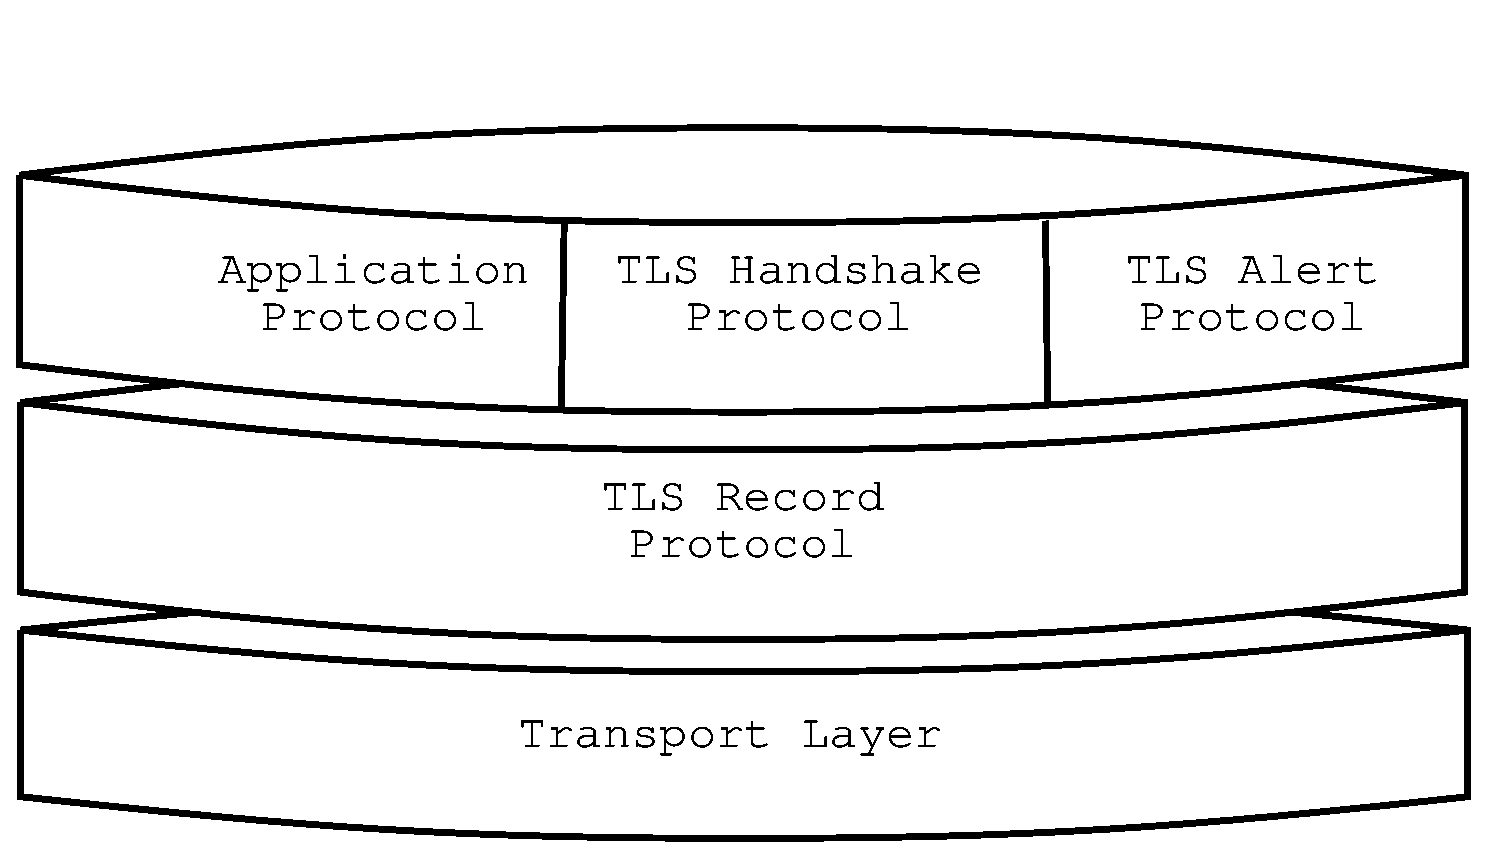
\includegraphics[height=8cm,width=12cm]{layers}
\label{fig:layers}
\caption{Layers in the TLS protocol}
\end{figure}


\addvspace{1.5cm}

